\documentclass[aspectratio=169, dvipdfmx,12pt]{beamer}% dvipdfmxしたい
\usepackage{bxdpx-beamer}% dvipdfmxなので必要
\usepackage{pxjahyper}% 日本語で'しおり'したい
\usepackage{minijs}% min10ヤダ
\usepackage{otf}
\usepackage{hyperref}
\usepackage{multirow}
\usepackage{color}

\usepackage[absolute,overlay]{textpos}
\usepackage{tikz}
\usetikzlibrary{shadows}
\usetikzlibrary{shapes.arrows,shapes.callouts,calc}


\renewcommand{\kanjifamilydefault}{\gtdefault}% 既定をゴシック体に
\pdfstringdefDisableCommands{%
  \def\CID{}%
}% "髙"によるエラー防止(author)

\newcommand<>{\PutAt}[3][0pt]{%
{\only#4{\begin{textblock*}{#1}#2%
  #3
\end{textblock*}}}%
}

\newcommand{\ShowPutAtGrid}{
  \begin{textblock*}{128mm}(0cm,0cm)
  \tikz[color=red!20!white]\draw[very thin, step=5mm] (0mm,0mm) grid (130mm,100mm);
  \end{textblock*}
  \begin{textblock*}{128mm}(0cm,0cm)
  \begin{tikzpicture}[color=red]
    \draw[step=1cm] (0,0mm) grid (130mm,100mm);   
    \foreach \n in {0,...,12}
      \draw[xshift=.5mm,yshift=-1.5mm, inner sep=0pt, anchor=west] (\n,10) node {\scriptsize{\textbf{\n}}};
    \foreach \n in {1,...,9}
      \draw[xshift=.5mm,yshift=-1.5mm, inner sep=0pt, anchor=west] (0,10-\n) node {\scriptsize{\textbf{\n}}};
  \end{tikzpicture}
  \end{textblock*}
}

\newcommand<>{\NormalBox}[2][]{%
  \only#3{\tikz[#1, every node/.style={shape=rectangle,draw,fill=white, drop shadow, #1}]\node []{#2};}
}

\newcommand<>{\OrangeBox}[2][]{%
  \onslide#3{\NormalBox[fill=orange!30,draw=black!30,rounded corners=4pt,#1]{#2}}%
} 


\usetheme{CambridgeUS}

\title{模型自動車を用いた遠隔型実車運転システム}
\author{\CID{8705}橋尚太郎}
\date[2021/12/1]{2021 12/1}
\institute[明石高専]{電気情報工学科 電気電子工学コース5年}
% [..]に省略名が書ける

\begin{document}
% \usebackgroundtemplate{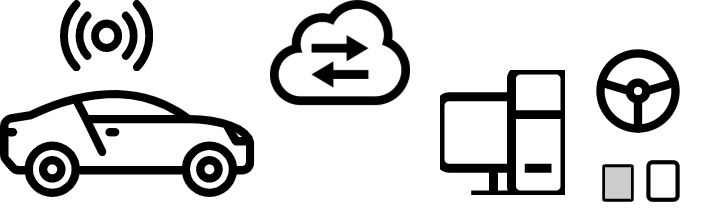
\includegraphics[width=\paperwidth]{img/remote_driving.png}}
\frame{\maketitle}
\begin{frame}{発表構成}
  \begin{columns}
    \begin{column}{0.5\textwidth}      
      \begin{enumerate}
        \item はじめに
        \item 遠隔型自動運転に関する制約
        \item 提案
        \item 目標設定
        \item 実装
        \item 実験
        \item 結果
        \item おわりに
      \end{enumerate}
    \end{column}
    
    \begin{column}{0.5\textwidth}
      \begin{figure}
        \centering
        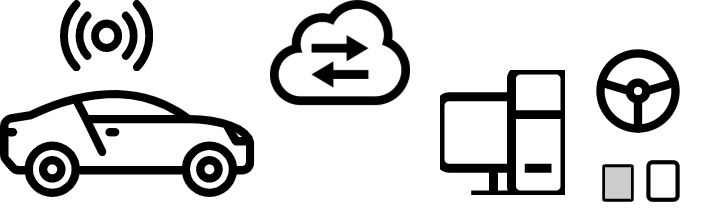
\includegraphics[width=0.8\textwidth]{img/remote_driving.png}
        \caption{A figure that is next to a certain explanation.}
      \end{figure}
    \end{column}
  \end{columns}
\end{frame}

\begin{frame}{はじめに}
  \begin{columns}
    \column{.51\textwidth}
      \vspace{-5truemm}%% スペース稼ぎ
      \begin{block}{自動運転技術}
        \begin{itemize}
          \item 2020年実用化に向けた法整備
          \item レベル3自動運転の解禁により遠隔型自動運転に注目
        \end{itemize}
      \end{block}
    \column{.47\textwidth}
    \begin{figure}
      \centering
      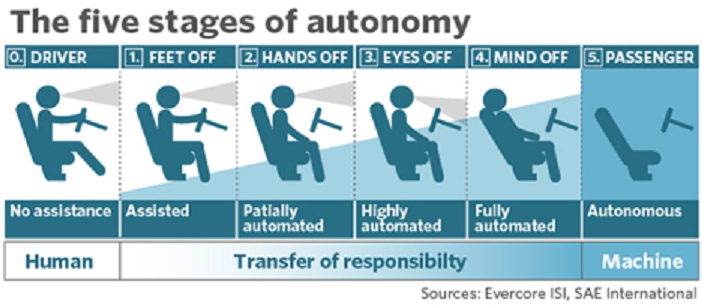
\includegraphics[width=0.95\textwidth]{img/stagesofautonomy.png}
      \vspace{-4truemm}
      \caption{Stages of Autonomy}
    \end{figure}
  \end{columns}

  \begin{block}{遠隔化}
    \begin{itemize}
      \item 自動運転レベル3以上に必須
      \item 異常時に遠隔操縦に切替
      \item 遠隔型自動運転:ドライバーが遠隔地から車側のリアルタイム映像を見ながら操縦
      \item 都市部から地方への移動サービス提供
    \end{itemize}
  \end{block}
\end{frame}

\begin{frame}{遠隔型自動運転に関する制約}
  \begin{columns}
    \column{.49\textwidth}
    \begin{block}{自動運転の補助にも免許が必須}
      \begin{itemize}
        \item 法基準で自動車免許と遠隔運転用の特殊な訓練が義務付けられている.
      \end{itemize}
    \end{block}
    \column{.45\textwidth}
    {\fontsize{7pt}{1pt}\selectfont 
    自動運転の公道実証実験に係る道路使用許可基準\\}
    {\fontsize{7pt}{1pt}\selectfont
    (3)安全確保措置\\
    ア 共通事項\\
    ウ 監視・操作が困難な状態となり得ることを踏まえた安全対策が盛り込まれた実施計画であること\\
    安全対策の例 他の監視・操作者となる者が速やかに監視・操作を後退できる体制をとる.\\
    (5)監視・操作者となる者\\
    イ 実験車両に応じ,必要な運転免許\\
    \vspace{-2mm}(仮運転免許を除く)を受けていること}
  \end{columns}
  \begin{columns}
    \column{.49\textwidth}
    \begin{block}{複数人での管理が必須}
      \begin{itemize}
        \item 東急バス実証実験(2020/12/17~2020/12/25)遠隔運転の特殊な訓練を受けた3人態勢で監視,操縦
      \end{itemize}
    \end{block}
    \column{.49\textwidth}
    \begin{figure}
      \centering
      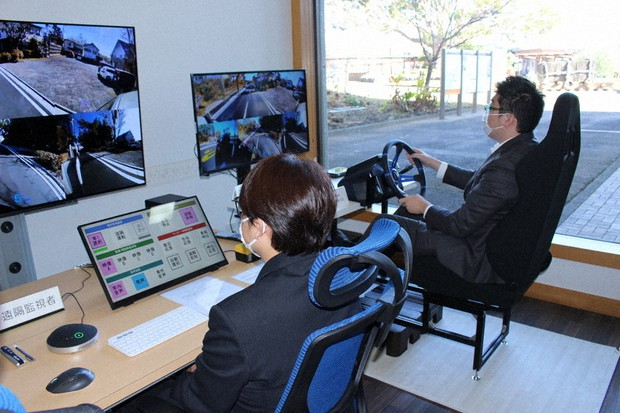
\includegraphics[width=0.8\textwidth]{img/tokyu1mainichi.jpg}
      \vspace{-3truemm}
      \caption{Experiment View of Remote Driving System}
    \end{figure}
  \end{columns}
\end{frame}

\begin{frame}{提案}
  \begin{block}{免許や法定の訓練が遠隔運転に必要}
  \end{block}
  \begin{columns}
    \begin{column}{.7\textwidth}
      \qquad\tikz{
              \draw[line width=1mm,-stealth] (0, 0) -- (0,-0.5);
                 }%
      \end{column}%
  \end{columns}
  \vspace{-4mm}
  \begin{columns}
    \column{.47\textwidth}
    \begin{block}{不要な実験環境があれば・・・}
      \begin{itemize}
        \item 遠隔運転システム特性調査
        \item システム開発
        \item 実務への適性調査の環境
      \end{itemize}
      として手軽に利用できる.
    \end{block}
    \column{.47\textwidth}
    \begin{figure}
      \centering
      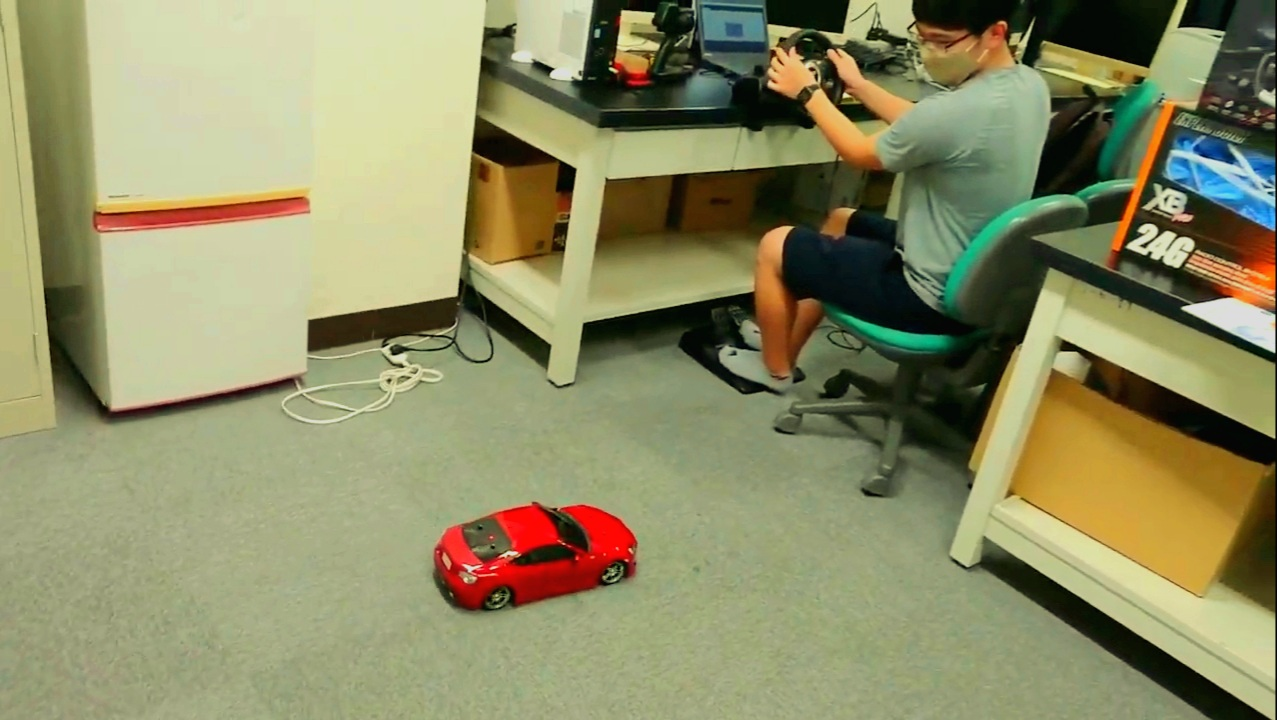
\includegraphics[width=0.9\textwidth]{img/driving_rds.jpg}
      \vspace{-3truemm}
      \caption{Ideal System}
    \end{figure}
  \end{columns}
  \vspace{-2mm}
  \begin{columns}
    \begin{column}{.7\textwidth}
      \qquad\tikz{
        \draw[line width=1mm,-stealth] (0, 0) -- (0,-0.5);
           }%
    \end{column}
  \end{columns}
  \begin{block}{本研究で提案}
    RCカーを用いた遠隔型実車運転システム
  \end{block}
\end{frame}

\begin{frame}{目標設定}
  \begin{block}{研究目的}
    \begin{itemize}
      \item 運転免許の所持不所持に関わらず,遠隔運転の実験に携わることが可能な練習及び研究のための環境を構築する.
      \item リアルタイム映像を見ながらハンドルとフットペダルで操作可能なRCカーの実現
    \end{itemize}
  \end{block}
  \begin{block}{研究の位置付け}
    \begin{itemize}
      \item 実験プロトタイプの提案
      \item 実装と走行実験で目的にアプローチ
    \end{itemize}
  \end{block}
\end{frame}

\begin{frame}{実装}

  \begin{columns}
    \centering
    \begin{column}{.3\textwidth}
      \begin{block}{操作視点の提供}
      \end{block}
    \end{column}
    \begin{column}{.2\textwidth}
      \qquad\tikz{
        \draw[line width=1mm, -stealth] (-0.5, -1) -- (0.5,-1);
           }%
    \end{column}
    \begin{column}{.3\textwidth}
      カメラ映像の,\\リアルタイム取得
    \end{column}
  \end{columns}
  \vspace{4mm}

  \begin{columns}
    \centering
    \begin{column}{.3\textwidth}
      \begin{block}{操作の無線化}
      \end{block}
    \end{column}
    \begin{column}{.2\textwidth}
      \qquad\tikz{
        \draw[line width=1mm, -stealth] (-0.5, -1) -- (0.5,-1);
           }%
    \end{column}
    \begin{column}{.3\textwidth}
      シリアル通信
    \end{column}
  \end{columns}
  \vspace{4mm}

  \begin{columns}
    \centering
    \begin{column}{.3\textwidth}
      \begin{block}{模型自動車の動作}
      \end{block}
    \end{column}
    \begin{column}{.2\textwidth}
      \qquad\tikz{
        \draw[line width=1mm, -stealth] (-0.5, -1) -- (0.5,-1);
           }%
    \end{column}
    \begin{column}{.3\textwidth}
      モータの回転制御
    \end{column}
  \end{columns}
\end{frame}

\begin{frame}{使用機材}
  \centering
  \begin{table}
    \caption{Using Equipment}
    \scalebox{0.8}{
    \begin{tabular}{cc}
    \hline
      機器 & 製品名 \\ 
      \hline \hline
      RCカー & TAMIYA 1/10 XB シリーズ TOYOTA 86 \\
      PC & Lenovo ThinkPad X240 \\
      ステアリングコントローラ & Logicool GT Force Pro \\
      ゲームパッドコントローラ & Dualshock3 \\
      マイコン & Arduino \\
      無線モジュールシールド & XBee Wireless Proto Shield \\
      無線モジュール & XBee S2C \\
      カメラ & GoPro MAX \\
      USB WiFi アダプタ & BUFFALOI-U2433DHP \\
      \hline
    \end{tabular}
    }
  \end{table}
\end{frame}

\begin{frame}{実装の詳細}
  
  \begin{columns}
    \begin{column}{0.5\textwidth}
      \begin{figure}
        % \centering
        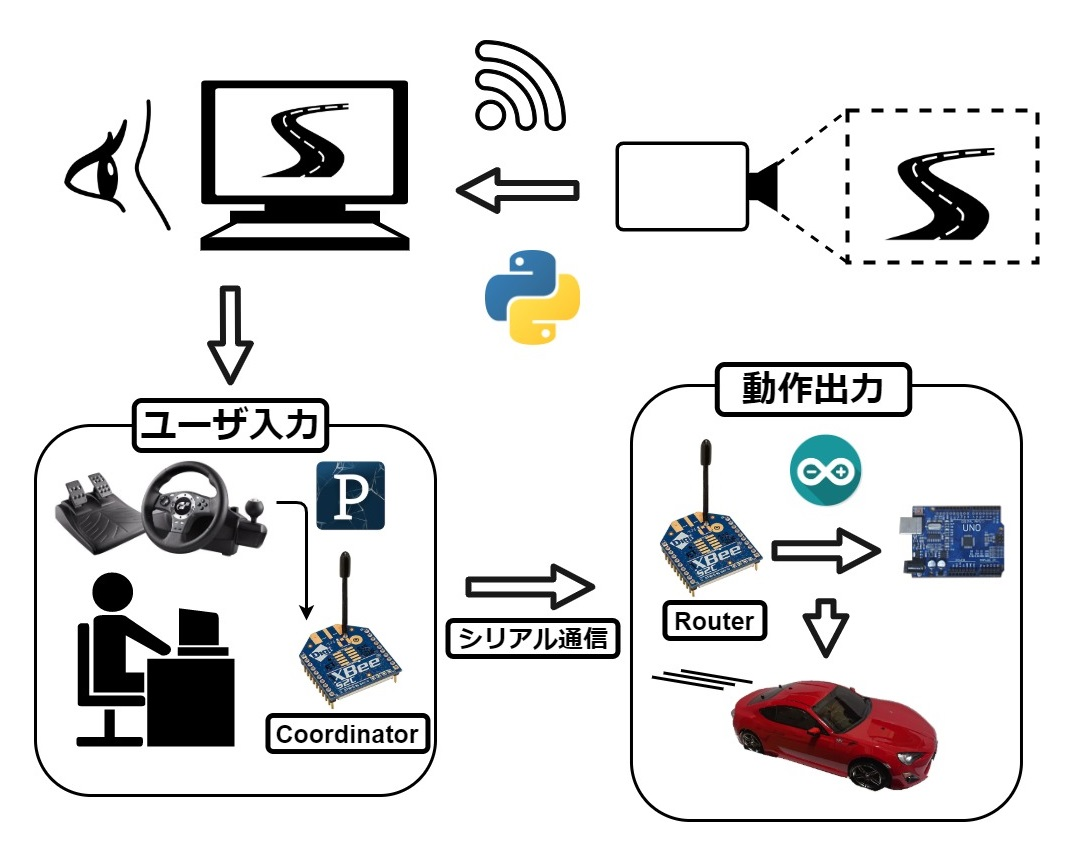
\includegraphics[width=1.0\textwidth]{img/operation.jpg}
        \caption{Function}
      \end{figure}
    \end{column}
    
    \begin{column}{0.35\textwidth}
      \begin{block}{カメラ映像の\\リアルタイム取得}
        \begin{itemize}
          \item OpenCV gopro-py
        \end{itemize}
      \end{block}
      \begin{block}{シリアル通信}
        \begin{itemize}
          \item Processing, Arduino, XBee
        \end{itemize}
      \end{block}
      \begin{block}{モータの回転制御}
        \begin{itemize}
          \item Arduino
        \end{itemize}
      \end{block}
      
      % \PutAt<+>{(8cm,2cm)}{
      %  \OrangeBox[text width=4cm, font=\footnotesize]{WiFi間でリアルタイム映像をPCに投影}
      %  \OrangeBox[text width=4cm, font=\footnotesize]{XBeeモジュール間のシリアル通信で制御信号をRCに送信}
      %}
    \end{column}

  \end{columns}

\end{frame}

\begin{frame}{操作方法}
  \begin{block}{ハンドル}
    \begin{itemize}
      \item 左右旋回
    \end{itemize}
  \end{block}
  \begin{block}{アクセルペダル}
    \begin{itemize}
      \item 前進
    \end{itemize}
  \end{block}
  \begin{block}{ブレーキペダル}
    \begin{itemize}
      \item 減速(1回踏む)
      \item 後退(2回踏んで踏み続ける)
    \end{itemize}
  \end{block}
\end{frame}

\begin{frame}{操作の仕組み(ハンドル)}
  \begin{figure}
    % \centering
    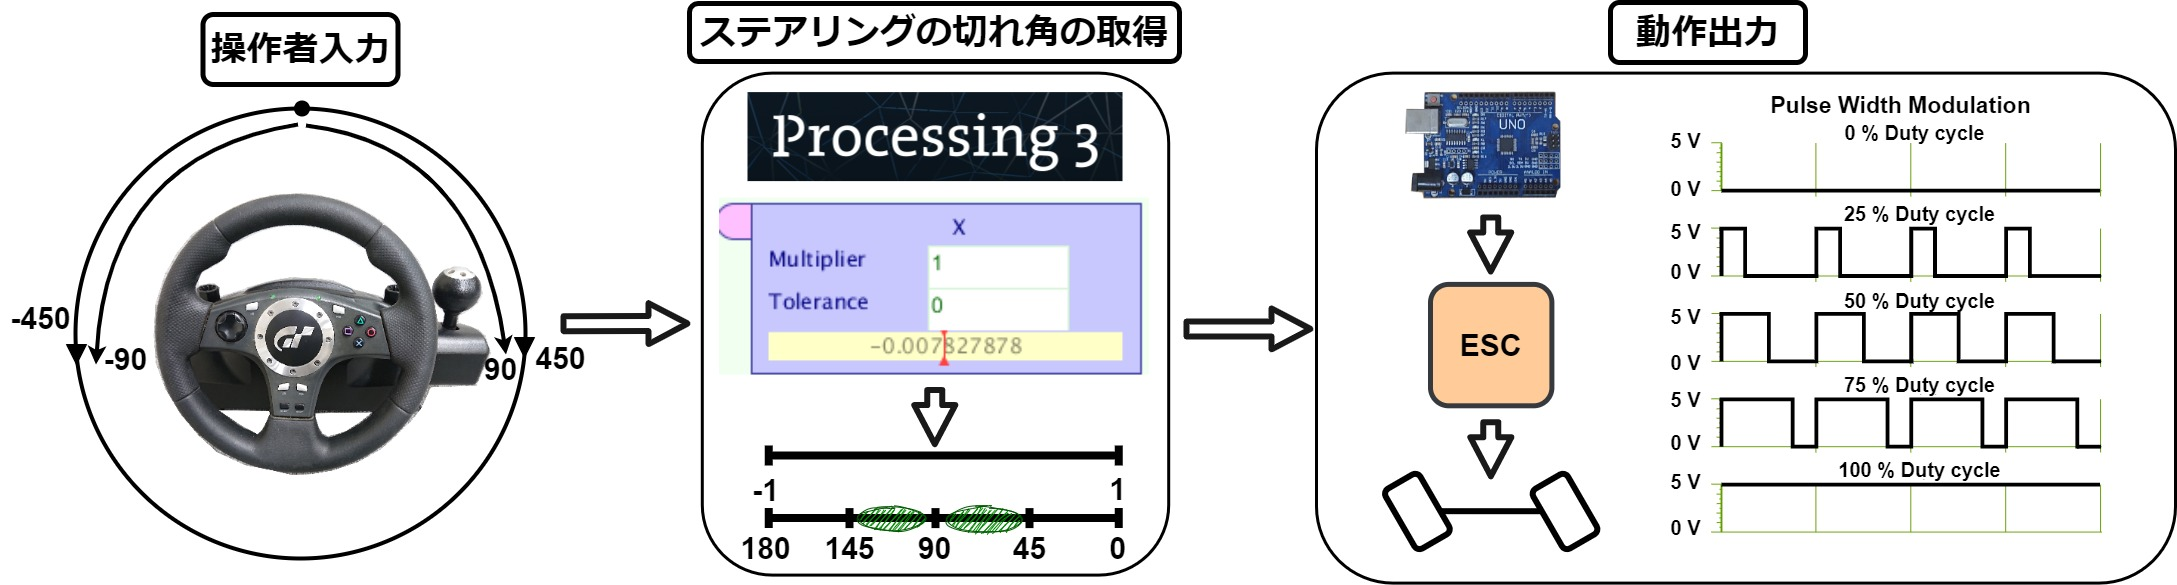
\includegraphics[width=1.0\textwidth]{img/steering.jpg}
    \vspace{-5truemm}
    \caption{Steering Function}
  \end{figure}

\end{frame}

\begin{frame}{操作の仕組み(スロットル)}
  \begin{figure}
    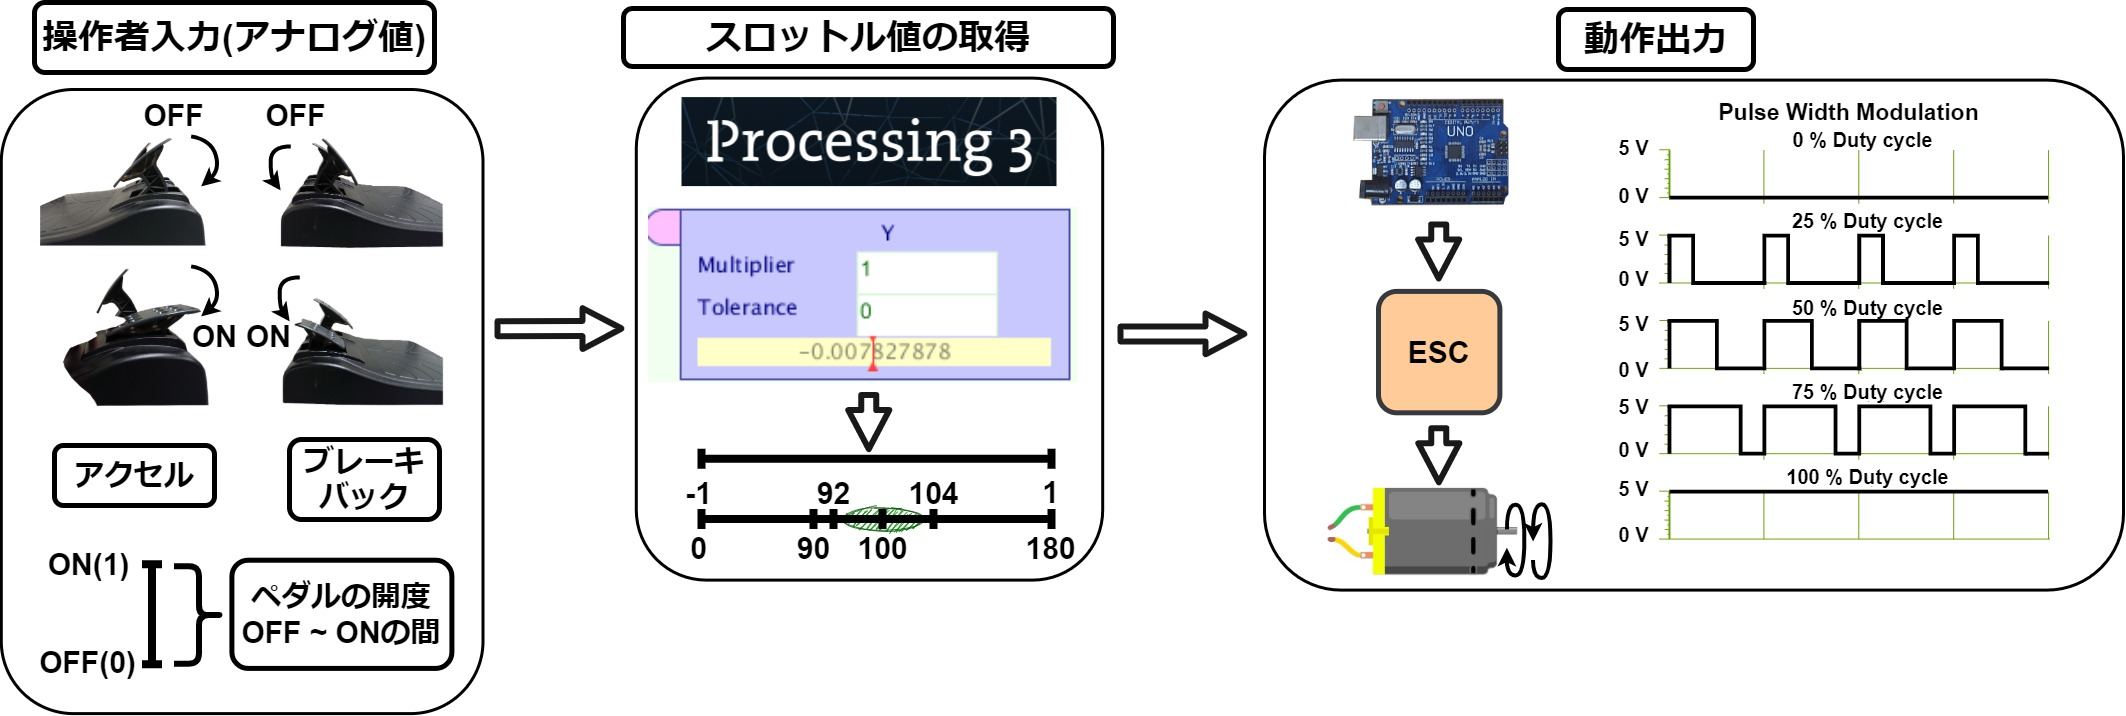
\includegraphics[width=1.0\textwidth]{img/throttle.jpg}
    \vspace{-5truemm}
    \caption{Throttle Function}
  \end{figure}
\end{frame}

\begin{frame}{ハードウェア}
  \begin{figure}
    \includegraphics[width=1.0\textwidth]{img/whole.png}
    \caption{Hardware Specification}
  \end{figure}
  \begin{block}{ESC(Electric Speed Controller)}
    ラジコン用のモータ制御回路\\
    ArduinoからESCを介してモータを制御
  \end{block}
\end{frame}

\begin{frame}{実験}
  \begin{block}{期待されるデータ}
    \begin{itemize}
      \item インターフェース操作の機敏性と正確性に関する比較結果
    \end{itemize}
  \end{block}
  \vspace{-2mm}
  \begin{block}{方法}
    \begin{itemize}
      \item 被験者によるコース周回走行
    \end{itemize}
    \begin{enumerate}
      \item ラップタイム測定(機敏性)
      \item 操作中の壁面等接触回数の記録(正確性)
      \item アンケート(被験者の体感情報: 操作感覚等)
    \end{enumerate}
  \end{block}
  \vspace{-2mm}
  \begin{block}{条件}
    \begin{enumerate}
      \item 被験者の実車運転経験:有,無
      \item 走行するコースの環境:操作自由度の高,低
      \item インターフェース:ハンドル・ペダル,プロポ,ゲームパッド
      \item 操作視点(1人称,3人称)
    \end{enumerate}
  \end{block}

\end{frame}

\begin{frame}{条件について}

  \begin{columns}
    \begin{column}{0.5\textwidth}
      \begin{figure}
        % \centering
        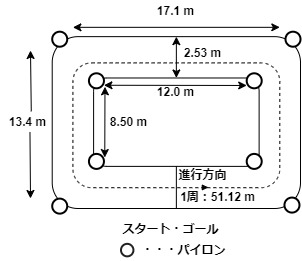
\includegraphics[width=0.5\textwidth]{img/course1.jpg}
      \end{figure}
    \end{column}

    \begin{column}{0.5\textwidth}
      \begin{figure}
        % \centering
        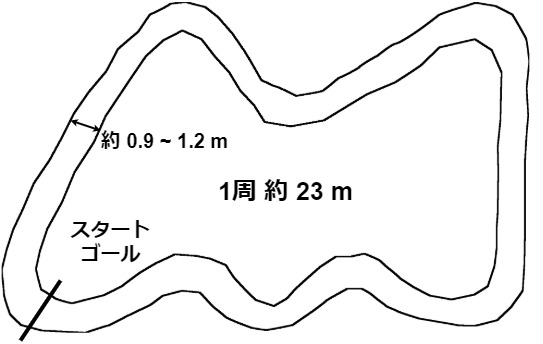
\includegraphics[width=0.5\textwidth]{img/course2.jpg}
      \end{figure}  
    \end{column}
  \end{columns}

  \begin{columns}
    \begin{column}{0.45\textwidth}
      \vspace{-6mm}
      \begin{block}{操作自由度が高い環境}
        \begin{itemize}
          \item 壁面なし
          \item 被験者5人(内1名2回) 6パターン
          \item ラップタイム測定\\(3周:1セット/被験者)
          \item アンケート(被験者主観)
        \end{itemize}
      \end{block}
    \end{column}

    \begin{column}{0.45\textwidth}
      \vspace{-11truemm}
      \begin{block}{操作自由度が低い環境}
        \begin{itemize}
          \item 壁面あり
          \item 被験者3人 3パターン
          \item ラップタイム測定\\(3周:2セット/被験者)
          \item アンケート(被験者主観)
        \end{itemize}
      \end{block}
    \end{column}
  \end{columns}

\end{frame}

\begin{frame}

  \begin{columns}
    \begin{column}{0.5\textwidth}
      \begin{figure}
        % \centering
        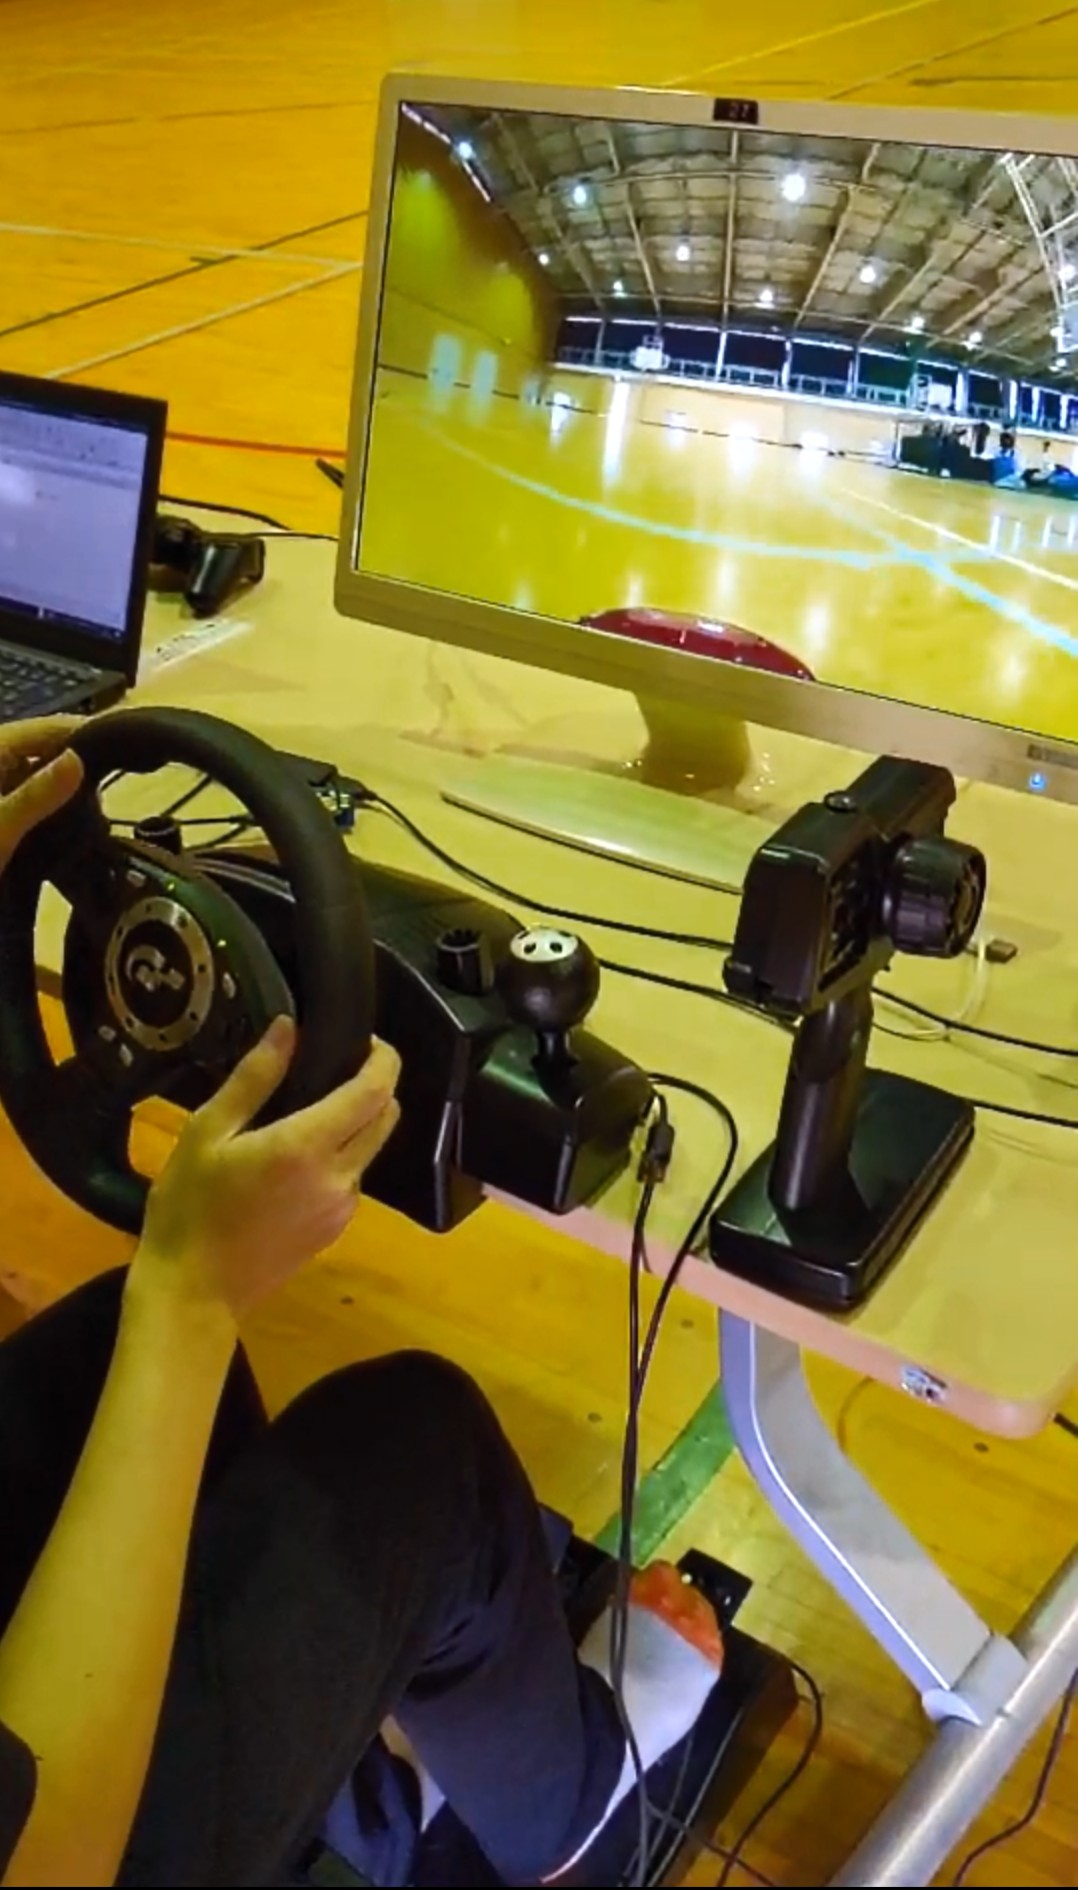
\includegraphics[width=0.6\textwidth]{img/rds.JPG}
        \caption{The view of cockpit (first person)}
      \end{figure}
    \end{column}
    
    \begin{column}{0.5\textwidth}
      \begin{figure}
        % \centering
        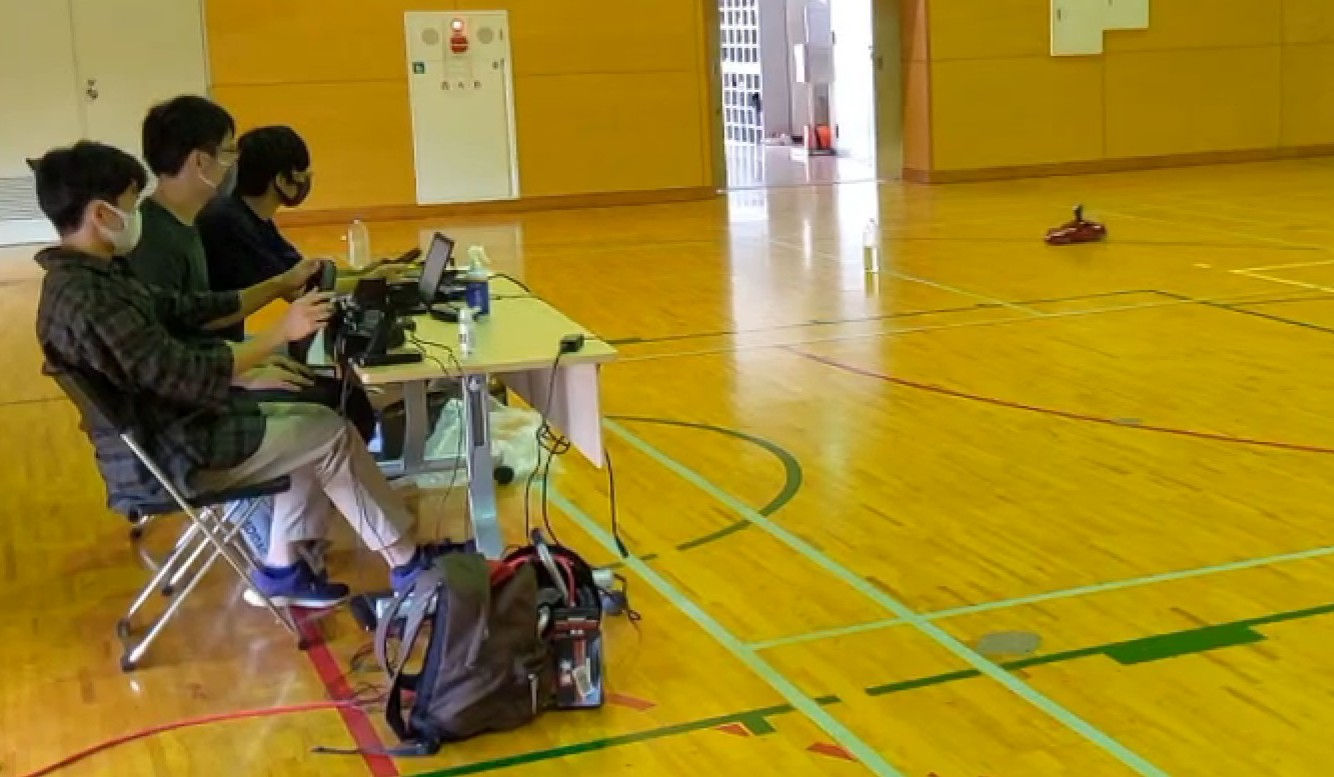
\includegraphics[width=0.8\textwidth]{img/three.JPG}
        \caption{The direct view (third person) }
        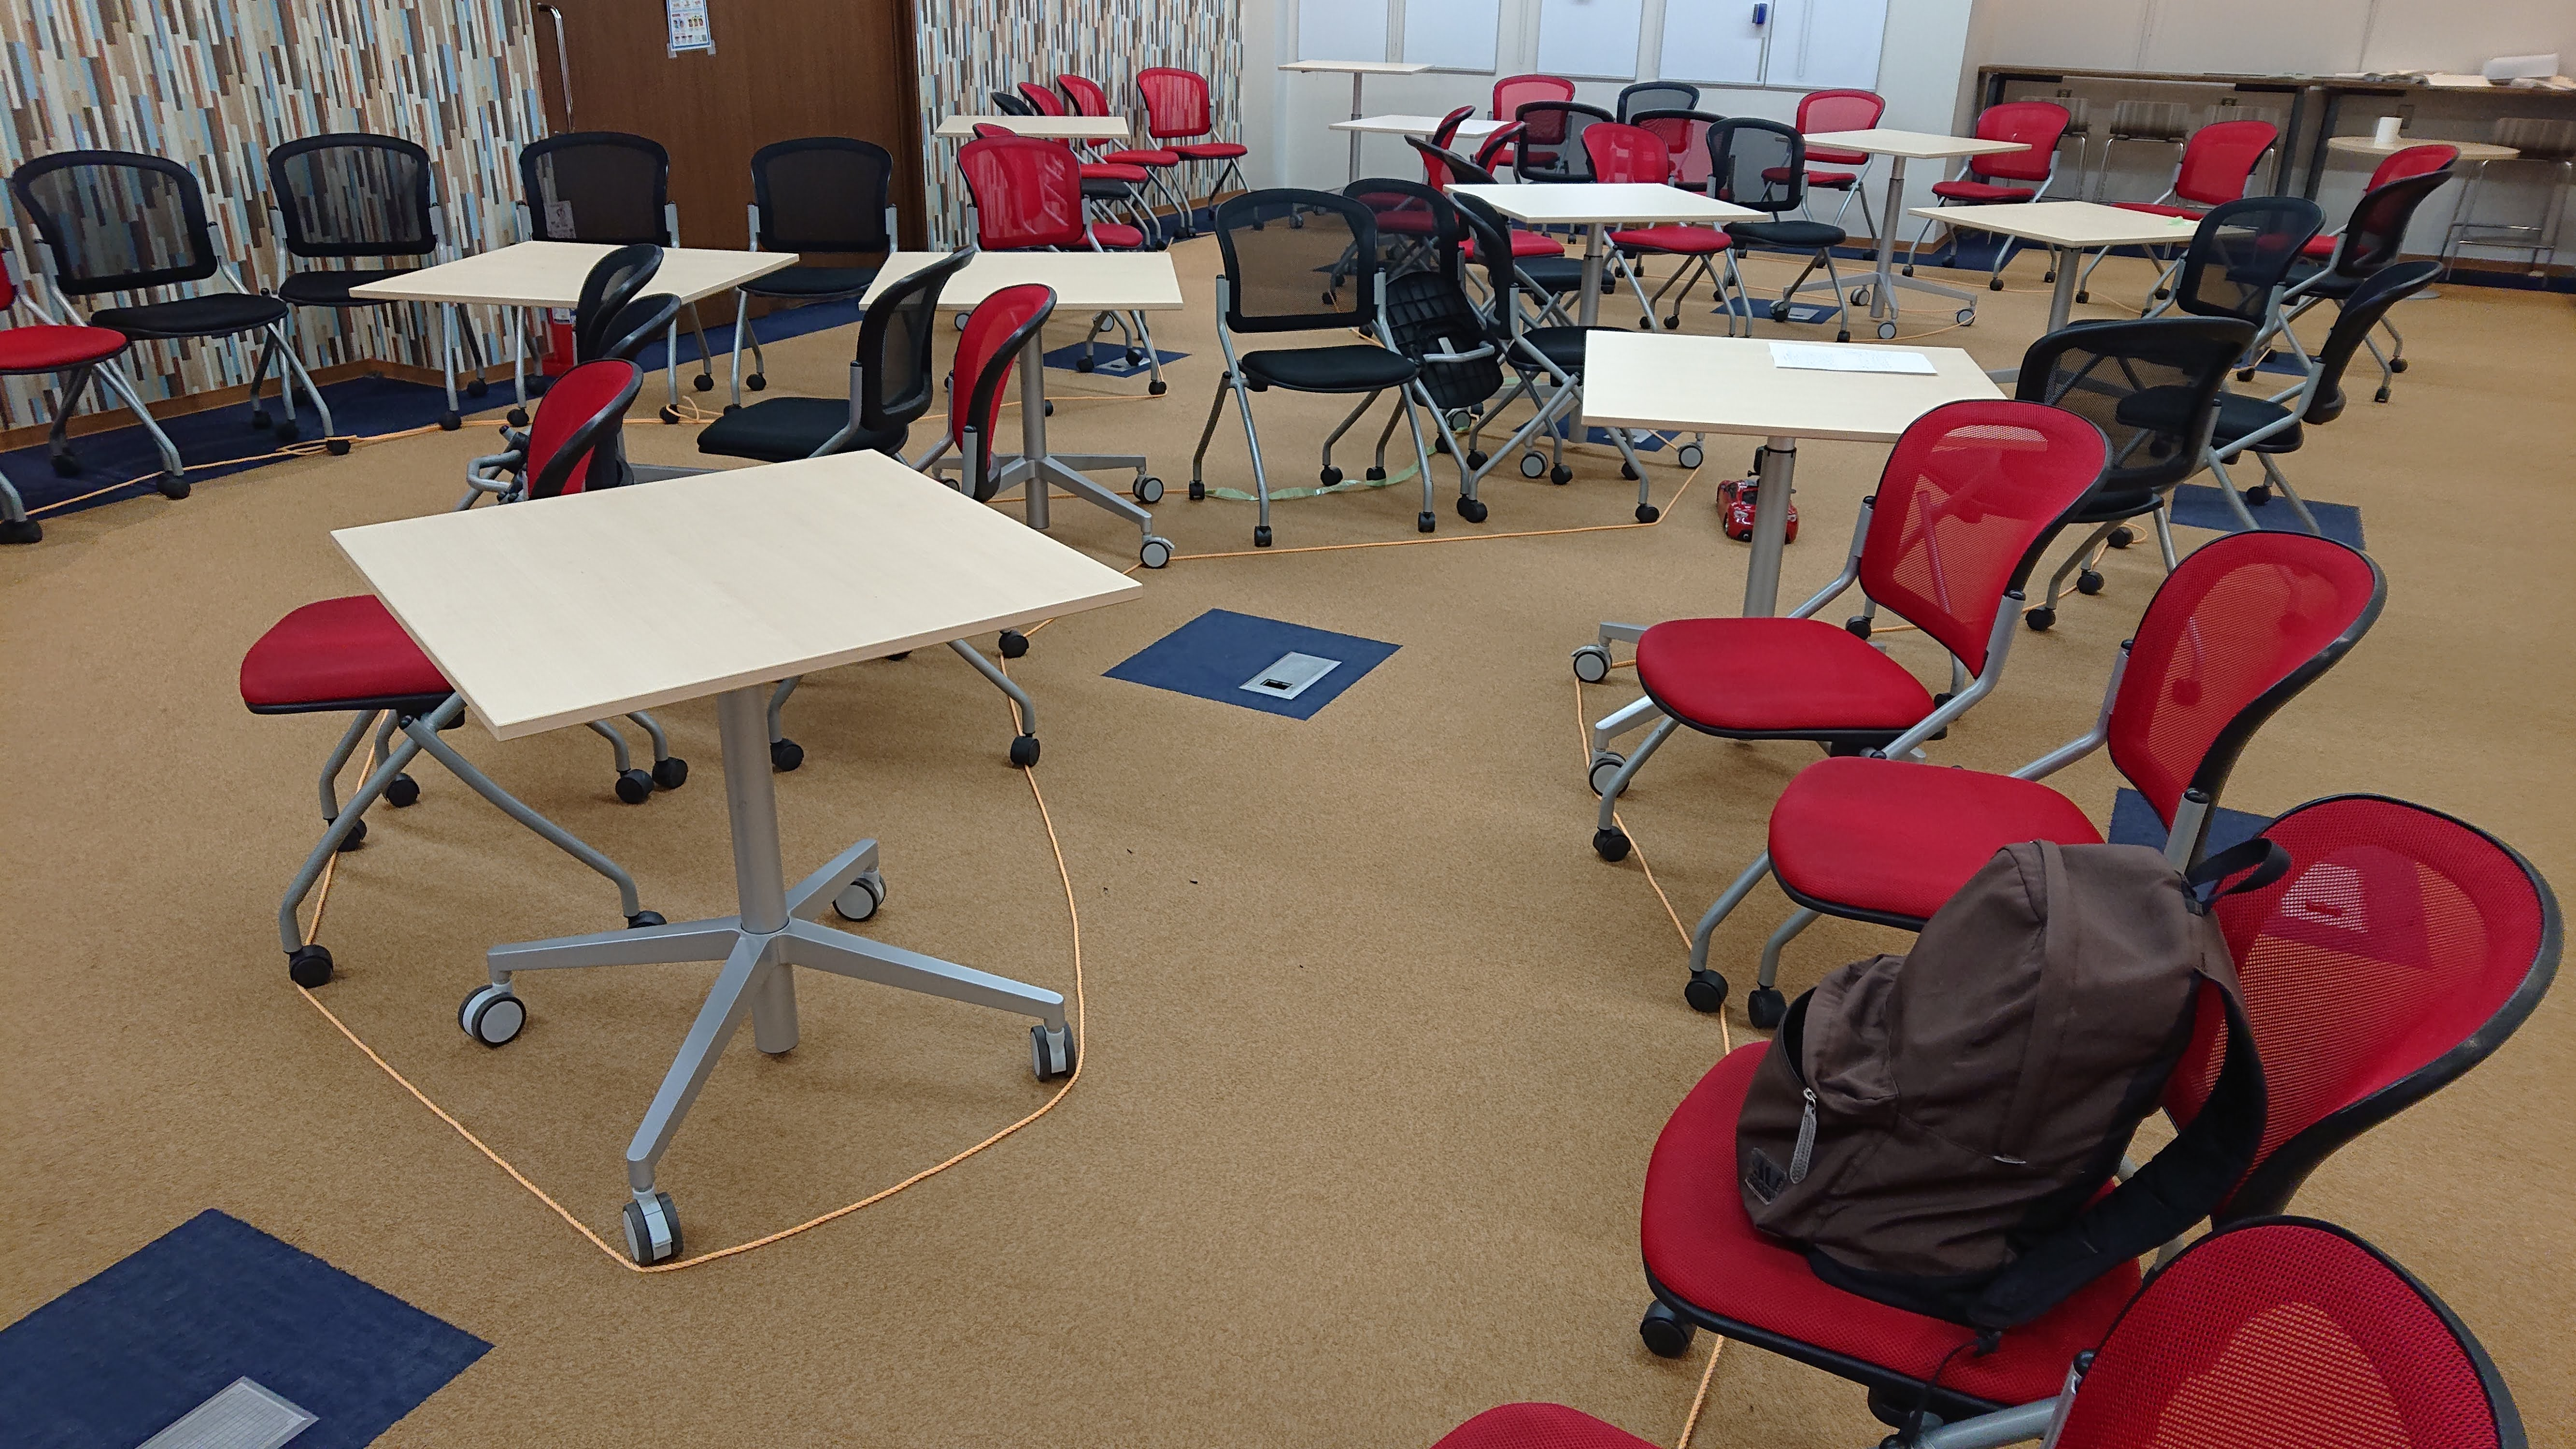
\includegraphics[width=0.8\textwidth]{img/course.jpg}
        \caption{narrow course}
      \end{figure}
    \end{column}
  \end{columns}

\end{frame}

\begin{frame}{実験結果}
  \begin{columns}
    \begin{column}{0.47\textwidth}
      \begin{block}{ラップタイムの比較}
        \begin{enumerate}
          \item 実車運転経験:差異なし
          \item 操作自由度:高い環境が優
          \item インターフェース:ゲームパッドが約10\%優
          \item 操作視点:目視 約10\%優
        \end{enumerate}
      \end{block}
    \end{column}

     \begin{column}{0.47\textwidth}
      \begin{block}{接触回数等の比較}
        \begin{enumerate}
          \item 実車運転経験:有経験者が50\%以上少
          \item インターフェース:ゲームパッドが約10~23\%優
        \end{enumerate}
      \end{block}
    \end{column}
  \end{columns}

  \begin{columns}
    \begin{column}{0.8\textwidth}
      \begin{block}{アンケート}
        \begin{enumerate}
          \item 実車運転経験:優経験者の方が慎重な運転の傾向
          \item 操作自由度:低い環境だと操作難化⇒映像遅延
          \item インターフェース:ゲームパッドが最適
          \item 操作視点:カメラより目視の方が良い
        \end{enumerate}
      \end{block}
    \end{column}
  \end{columns}
\end{frame}

\begin{frame}{接触箇所}

  \vspace{-5truemm}
  \begin{columns}
    \begin{column}{0.34\textwidth}
      \begin{figure}
        % \centering
        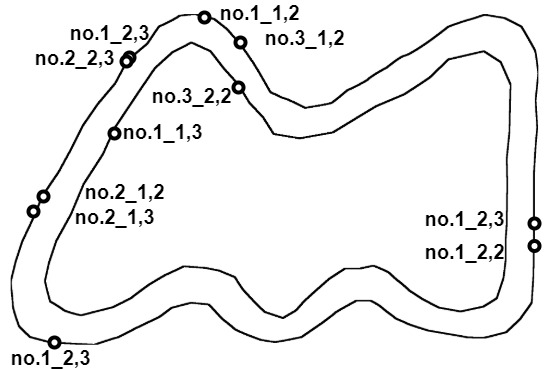
\includegraphics[width=1.0\textwidth]{img/gamepad_exp.jpg}
      \end{figure}
    \end{column}

    \begin{column}{0.34\textwidth}
      \begin{figure}
        % \centering
        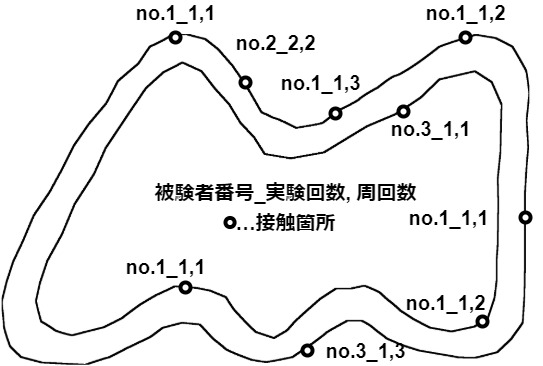
\includegraphics[width=1.0\textwidth]{img/steering_exp.jpg}
      \end{figure}  
    \end{column}

    \begin{column}{0.34\textwidth}
      \begin{figure}
        % \centering
        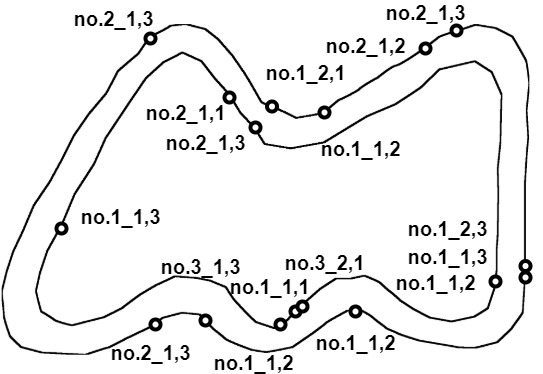
\includegraphics[width=1.0\textwidth]{img/propo_exp.jpg}
      \end{figure}
    \end{column}
  \end{columns}

  \begin{columns}
    \begin{column}{0.3\textwidth}
      \begin{block}{ゲームパッド操作}
        \begin{itemize}
          \item 特定の箇所に集中
        \end{itemize}
        \end{block}
      \end{column}
  
    \begin{column}{0.3\textwidth}
      \begin{block}{ハンドルペダル操作}
        \begin{itemize}
          \item コース全体に均一
        \end{itemize}
      \end{block}
    \end{column}
  
    \begin{column}{0.3\textwidth}
      \begin{block}{プロポ操作}
       \begin{itemize}
        \item 接触回数が最も多い
       \end{itemize}
      \end{block}
    \end{column}
  \end{columns}

\end{frame}

\begin{frame}{接触回数の遷移}
  \begin{columns}
    \begin{column}{0.3\textwidth}
      \begin{block}{1セット目}
        \begin{itemize}
          \item ハンドル:8回
          \item プロポ:15回
          \item パッド:5回
        \end{itemize}
      \end{block}
    \end{column}

    \begin{column}{.1\textwidth}
      \qquad\tikz{
        \draw[line width=1mm, -stealth] (-0.5, -1) -- (0.5,-1);
           }%
    \end{column}

     \begin{column}{0.3\textwidth}
      \begin{block}{2セット目}
        \begin{itemize}
          \item ハンドル:1回
          \item プロポ:9回
          \item パッド:18回
        \end{itemize}
      \end{block}
    \end{column}
  \end{columns}

  \begin{columns}

    \begin{column}{0.43\textwidth}
      \begin{block}{2セット目/1セット目(\%)}
        \begin{enumerate}
          \item ハンドル:12.5\%
          \item プロポ:60\%
          \item パッド:360\%
        \end{enumerate}
      \end{block}
    \end{column}

    \begin{column}{0.4\textwidth}
      \OrangeBox[text width=5cm]{ハンドルフットペダルが\\最も習熟しやすい\\インターフェース}
    \end{column}

  \end{columns}
\end{frame}

\begin{frame}{走行速度}

  \vspace{-5truemm}
  \begin{columns}
    \begin{column}{0.5\textwidth}
      \begin{figure}
        % \centering
        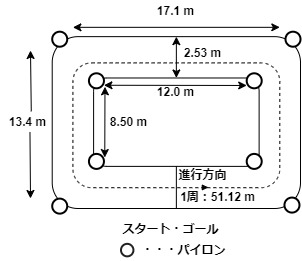
\includegraphics[width=0.75\textwidth]{img/course1.jpg}
      \end{figure}
    \end{column}

    \begin{column}{0.5\textwidth}
      \begin{figure}
        % \centering
        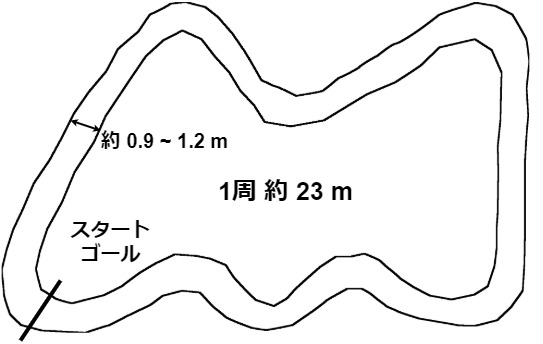
\includegraphics[width=0.75\textwidth]{img/course2.jpg}
      \end{figure}  
    \end{column}
  \end{columns}

  \begin{columns}
    \begin{column}{0.45\textwidth}
      \vspace{-6truemm}
      \begin{block}{操作自由度が高い環境}
        \begin{itemize}
          \item 実速度:約 5 ~ 8 km/h
          \item スケールスピード:\\ 約 16 ~ 25 km/h
        \end{itemize}
      \end{block}
    \end{column}

     \begin{column}{0.45\textwidth}
      \vspace{-6truemm}
      \begin{block}{操作自由度が低い環境}
        \begin{itemize}
          \item 実測度:約 2 ~ 3 km/h
          \item スケールスピード:\\ 約 6 ~ 10 km/h
        \end{itemize}
      \end{block}
    \end{column}
  \end{columns}

\end{frame}

\begin{frame}{アンケート結果}
  \begin{columns}
    \begin{column}{1.0\textwidth}
      \begin{table}
        \caption{Questionnaire Result}
        \scalebox{0.6}{
        \begin{tabular}{|c|c|}
        \hline
          設問 & 解答 \\ \hline
          実車運転経験 & あり:1 なし:2 \\ \hline
          操作感覚が実車に似ている & どちらとも言えない:1 \\ \hline
          実車より運転が簡単 & やや当てはまる:1 \\ \hline
          運転に対する苦手意識 & ない:2 ある:1 \\ \hline
          具体的な苦手意識 & "他の物体との接触" \\ \hline
          遠隔運転後,苦手意識の変化 & 変化なし:1 \\ \hline
          実車意外の運転経験 & ゲームあるいは実車運転シミュレーション:3 \\ \hline
          \begin{tabular}{c}
            免許講習意外で実車を使う前に\\遠隔運転環境を使いたい\\または用いると便利か
          \end{tabular}
          & とても思う:1 そう思う:1 どちらとも言えない:1 \\ \hline
          操作時の視点の快適さ & カメラ映像を見る:2 RCカーを直接見る:2 \\ \hline
          \begin{tabular}{c}
            操作性が快適だと思った\\操作機器の順位付け  
          \end{tabular}
          & 1位ハンドル:3 2位プロポ:3 \\ \hline
        \end{tabular}
        }
      \end{table}
    \end{column}
  \end{columns}
\end{frame}

\begin{frame}{考察}
  \begin{block}{操作自由度の高いコース}
    \begin{itemize}
      \item 1人1セット走行:被験者を変えて実施
      \begin{itemize}
        \item 周回タイムはどの機器でも一定
      \end{itemize}
    \end{itemize}
  \end{block}
  \begin{columns}
    \begin{column}{.25\textwidth}
      \qquad\tikz{
              \draw[line width=1mm,-stealth] (0, 0) -- (0,-0.5);
                 }%
      \end{column}%
  \end{columns}
  \begin{block}{操作自由度の低いコース}
    \begin{itemize}
      \item 1人2セット走行:被験者を変えず実施
      \begin{itemize}
        \item 機器操作の頻度を増加
      \end{itemize}
    \end{itemize}    
  \end{block}
  \begin{columns}
    \begin{column}{.25\textwidth}
      \qquad\tikz{
              \draw[line width=1mm,-stealth] (0, 0) -- (0,-0.5);
                 }%
      \end{column}%
  \end{columns}
  \begin{block}{結果}
    \begin{itemize}
      \item ハンドルペダル操作の場合接触回数が\textcolor{red}{12.5\%}に減少
      \begin{itemize}
        \item \textcolor{red}{習熟によって操作精度が向上}
      \end{itemize}
    \end{itemize}
  \end{block}
\end{frame}

\begin{frame}{結論}
  \begin{block}{遠隔運転の練習は運転免許の有無によらず可能}
    \begin{itemize}
      \item 条件:5 km/h 以下,道幅4台,壁無
      \item ただし,カメラ映像遅延の影響が無視できない
    \end{itemize}
  \end{block}
  \vspace{-3mm}
  \begin{block}{実車経験・未経験両方にメリットあり}
    \begin{itemize}
      \item ハンドルに慣れやすい(未経験者)
      \item 苦手意識の軽減(経験者)
      \item 楽しい(両方)
    \end{itemize}
  \end{block}
  \vspace{-3mm}
  \begin{block}{実験を行う事で得られた新たな知見}
    \begin{itemize}
      \item 経験者:実車より簡単(ハンドル・ペダル)
      \item ハンドルペダル:\textcolor{red}{習熟によって操作精度が向上}
      \item ゲームパッド・プロポ:\textcolor{red}{周回増えると接触頻度増加}
    \end{itemize}
  \end{block}
\end{frame}

\begin{frame}{おわりに}
  \begin{block}{まとめ}
    \begin{itemize}
      \item 遠隔型実車運転システム→RCカーへの実装を提案
      \item 運転免許無でも遠隔運転の練習を体験できるシステムの構築
      \item システム操作による効果の報告
      \begin{itemize}
        \item 実験結果,新たな知見
      \end{itemize}
      \item 自由度高:RCカ―の最高速度,遅延→操作性に影響(タイム)
      \item 自由度低:被験者の操作機器への習熟感覚,遅延→操作性に影響(タイム,接触)
    \end{itemize}
  \end{block}
  \begin{block}{今後の課題}
    \begin{itemize}
      \item カメラ映像の低遅延化
      \item 高精度な車速制御機能の実装(e.x.ドライブアシスト機能)
    \end{itemize}
  \end{block}
\end{frame}

\end{document}